\documentclass[a4paper,man,apacite,natbib,12pt]{apa6}\usepackage[]{graphicx}\usepackage[]{color}
%% maxwidth is the original width if it is less than linewidth
%% otherwise use linewidth (to make sure the graphics do not exceed the margin)
\makeatletter
\def\maxwidth{ %
  \ifdim\Gin@nat@width>\linewidth
    \linewidth
  \else
    \Gin@nat@width
  \fi
}
\makeatother

\definecolor{fgcolor}{rgb}{0.345, 0.345, 0.345}
\newcommand{\hlnum}[1]{\textcolor[rgb]{0.686,0.059,0.569}{#1}}%
\newcommand{\hlstr}[1]{\textcolor[rgb]{0.192,0.494,0.8}{#1}}%
\newcommand{\hlcom}[1]{\textcolor[rgb]{0.678,0.584,0.686}{\textit{#1}}}%
\newcommand{\hlopt}[1]{\textcolor[rgb]{0,0,0}{#1}}%
\newcommand{\hlstd}[1]{\textcolor[rgb]{0.345,0.345,0.345}{#1}}%
\newcommand{\hlkwa}[1]{\textcolor[rgb]{0.161,0.373,0.58}{\textbf{#1}}}%
\newcommand{\hlkwb}[1]{\textcolor[rgb]{0.69,0.353,0.396}{#1}}%
\newcommand{\hlkwc}[1]{\textcolor[rgb]{0.333,0.667,0.333}{#1}}%
\newcommand{\hlkwd}[1]{\textcolor[rgb]{0.737,0.353,0.396}{\textbf{#1}}}%

\usepackage{framed}
\makeatletter
\newenvironment{kframe}{%
 \def\at@end@of@kframe{}%
 \ifinner\ifhmode%
  \def\at@end@of@kframe{\end{minipage}}%
  \begin{minipage}{\columnwidth}%
 \fi\fi%
 \def\FrameCommand##1{\hskip\@totalleftmargin \hskip-\fboxsep
 \colorbox{shadecolor}{##1}\hskip-\fboxsep
     % There is no \\@totalrightmargin, so:
     \hskip-\linewidth \hskip-\@totalleftmargin \hskip\columnwidth}%
 \MakeFramed {\advance\hsize-\width
   \@totalleftmargin\z@ \linewidth\hsize
   \@setminipage}}%
 {\par\unskip\endMakeFramed%
 \at@end@of@kframe}
\makeatother

\definecolor{shadecolor}{rgb}{.97, .97, .97}
\definecolor{messagecolor}{rgb}{0, 0, 0}
\definecolor{warningcolor}{rgb}{1, 0, 1}
\definecolor{errorcolor}{rgb}{1, 0, 0}
\newenvironment{knitrout}{}{} % an empty environment to be redefined in TeX

\usepackage{alltt}
\usepackage{../Common/style/Mason}
\usepackage{listings}
\usepackage{inconsolata}

%%%%%%%%%%%% Title %%%%%%%%%%%%
\title{Intelligence and Age at First Intercourse: Cause or Confound?}
\shorttitle{Intelligence and AFI}

% Authors and Affliations
\author{S. Mason Garrison and Joseph Lee Rodgers}
\affiliation{Vanderbilt University}

% Author Note
\authornote{{\small S. Mason Garrison, Department of Psychology and Human Development, Vanderbilt University; Joseph Lee Rodgers, Department of Psychology and Human Development, Vanderbilt University.

This manuscript is based on longitudinal data collected as part of the National Longitudinal Survey of Youth 1979, (NLSY79). These data are publicly available; a bibliography of articles using these surveys can be found at \url{https://nlsinfo.org/bibliography-start} This material is based upon work that has been supported by the National Institute of Health under Grant No. (R01-HD065865) and the National Science Foundation Graduate Research Fellowship Program under Grant No. (DGE-1445197), and various means of institutional support from the following universities: University of British Columbia, University of Oklahoma \& Vanderbilt University. The aforementioned funding sources did not have any input in the production of this article.

Correspondence concerning this article should be addressed to S. Mason Garrison, Department of Psychology and Human Development, Vanderbilt University, Nashville, TN. Contact: s.mason.garrison@gmail.com}
}

% Abstract
\abstract{Last compile was \today\ at \currenttime\\
%% Empirical Study
\input{../Common/content/title/abstract_empreport.txt}}
\IfFileExists{upquote.sty}{\usepackage{upquote}}{}
\begin{document}
\maketitle
%
%%%%%%%%%%%% R %%%%%%%%%%%%











%%%%%%%%%%%% Introduction %%%%%%%%%%%%
%\section{Introduction}
\section{ }\vspace{-.8cm}
% Introduce the Major Problem
\input{../Common/content/introduction/introduce_the_problem.txt}\\
\input{../Common/content/introduction/importance_of_problem.txt}

% Relevant Scholarship
%\subsection{Relevant Scholarship}
\input{../Common/content/introduction/relevant_scholarship.txt}\\

% Current Study
\subsection{Current Study}
To summarize, the current study examines the relationship between intelligence and age at first intercourse, using maternal siblings and their children from a multi-generational nationally representative sample, the NLSY. This examination extends the intelligence literature in several key ways. First, we test whether the relationship between intelligence and AFI existed in either or both between- and within-family analyses, using data in which we can explicitly separate those sources of variance. Second, we evaluated the alternative explanation that maternal intelligence influences child AFI, using the cross-generational structure of the NLSY. Third, we replicated our findings using two different age periods. Fourth, we address overlapping questions to those studied in Halpern \et (\citeyear{halpern2000smart}, Harden and Mendle (\citeyear{harden2011don}), and Nedelec \et (\citeyear{nedelec2012exploring}), using a different data source.\footnote{All of those previous studies used the Add Health dataset.}

We made the following predictions, based primarily upon \citet{harden2011don}:\\ 
Between Families,\\
1.\hypothesis{btw_2_2} Does Generation 2 (\ie, children's) intelligence predict Generation 2 AFI?: We expect intelligence to be associated with age of first intercourse because there is a sizable body of literature reporting that result \citep{kirby2002effective, manlove1998influence, raffaelli2003sexual, rodgers1994df}.\\ 
2.\hypothesis{btw_1_2} Does Generation 1 (\ie, mother's) intelligence predict Generation 2 AFI?: We also expect maternal intelligence to be associated with age of first intercourse because the heritability of intelligence is moderate-to-high \citep{Bouchard2004,devlin1997heritability}. If intelligence does causally influence AFI, we would expect that the cross-generational association between AFI and intelligence would be weaker, but existent. However, if the intelligence-AFI relationship is the product of between-family confounds, then we would expect that the cross-generational association between AFI and intelligence would be stronger than the within-generation association because maternal intelligence would be more closely linked with household SES and various parental causes. In other words, maternal intelligence can serve as a proxy for many of the between-family confounds that are of concern in the current study. Comparably sized effects would also be consistent with a between-family confound. Given that \citet{harden2011don} found no within-family effect for intelligence, we expect that maternal intelligence will have a comparable or larger effect on between-family AFI than child intelligence.\\
Within Families,\\
3.\hypothesis{wth_2_2} Does Generation 2 intelligence predict Generation 2 AFI?: We do not expect to find within-family differences in intelligence correlating with AFI, given that \citet{harden2011don} did not report an effect.\\
4.\hypothesis{wth_1_2} Does Generation 1 intelligence predict Generation 2 AFI?: Unknown -- it is possible that maternal intelligence will have an effect, as such a link would explain the between-family effects as well as many of the alternative household-level influences.\\
5.\hypothesis{btw_v_wth} Is the relationship consistent across cross-sectional and within-family designs?: Doubtful, we do not expect the results to be consistent across methods because both \citet{harden2011don} and \citet{Meredith2013} found no within-family effect, whereas the traditional findings from between-family studies find an effect \citep{kirby2002effective, manlove1998influence, raffaelli2003sexual}. The birth order literature is one example in which apparent causal links mitigate or disappear when variance is properly attributed to within- versus between-family sources.

%%%%%%%%%%%% Method %%%%%%%%%%%%
\section{Method}
% Research Design
\subsection{Research Design}
We adapted Kenny and colleagues \citeyearpar{kenny2001social,kenny2006dyadic} reciprocal standard dyad model to facilitate sibling comparisons. Sibling-based quasi-experimental models are particularly effective for incorporating genetic and environmental design elements \citep{Lahey2010,Rutter2007}. Our model uses differences between both pairs of mothers and pairs of adolescents, which provide the measures that explicitly account for within-family variance. Further, within-family differences create a powerful control for virtually all background heterogeneity (variance) associated with both genetic and environmental differences (\citeauthor{Lahey2010}). We compare individuals from within the family in the context of the following models. First, we predict the difference in AFI, $Y_{i\Delta}$, for a given pair of NLSY-Children, indexed as i, in the following model:
\begin{equation}\label{equation_discord_main}
\mathrm{Y_{i\Delta}} = \beta_0 + \beta_1\mathrm{\bar{Y_{i}}} + \beta_2\mathrm{\bar{X_{i}}} + \beta_3\mathrm{X_{i\Delta}}
\end{equation}\vspace{-10pt}
where,
\begin{equation}\label{equation_discord_defs_delta}
\mathrm{Y_{i\Delta}} = \mathrm{Y_{i1}} - \mathrm{Y_{i2}};\, \mathrm{X_{i\Delta}} = \mathrm{X_{i1}} - \mathrm{X_{i2}},\, \mathrm{and}
\end{equation}
\begin{equation}\label{equation_discord_defs_min}
\mathrm{Y_{i1}} = \mathrm{max}(\mathrm{Y_{ij}});\, \mathrm{Y_{i2}} = \mathrm{min}(\mathrm{Y_{ij}})
\end{equation}\\

In this model, the relative difference in kin outcomes ($\mathrm{Y_{\Delta}}$; \eg, AFI) is predicted from the mean level of Y ($\mathrm{\bar{Y}}$; \eg mean AFI), the mean level of X ($\mathrm{\bar{X}}$; \eg, intelligence), and the between-kin intelligence difference ($\mathrm{X_{i\Delta}}$). The mean levels, reflecting between-family variance, support causal inference through at least partial control for genes and shared environment in previous generations. Within this model, there is explicit separation of within-family variance (with $\mathrm{Y_{\Delta}}$ and $\mathrm{X_{\Delta}}$), and between-family variance (with $\mathrm{\bar{Y}}$ and $\mathrm{\bar{X}}$).

For our analytic models, we use either the complete version or subsets of this overall analytic model to achieve different goals (elaborated below).  We can use only the between-family independent variables, only the within-family independent variable, or both (the first and the third models achieve the goals of the current study).

Thus, this model explicitly untangles between- and within-family influences. If there is a true causal link between intelligence and AFI, then we expect kin differences in intelligence to be significantly associated with kin differences in AFI. If the effect is spurious -- only a function of between-family confounds -- then we would expect to find no significant relationship between the differences in the outcome with the differences in the predictor.
%
% Sample
\subsection{Sample}
The National Longitudinal Survey of Youth 1979 dataset(NLSY79) is based on a nationally representative household probability sample, jointly sponsored by the U.S. Bureau of Labor Statistics and the U.S. Department of Defense. On December 31, 1978, 12,686 adolescents were sampled within a household probability sample from 8,770 households. The initial sample consisted of three subsamples: \begin{itemize}\item a cross--sectional household probability sample of 6,111 non-institutionalized adolescents residing in the United States on December $31^{st}$ of 1978; \item a separate over-sampled civilian subsample of 5,295 racial minorities and disadvantaged whites; \item a representative sample of 1,280 youth serving in the U.S. Military on September $30^{th}$, 1978.\end{itemize} In the two civilian samples, subjects' birthdates ranged from January 1, 1957 to December 31, 1964, and were between the ages of 14 and 21 on December 31, 1978; military subject's birthdates ranged from January 1, 1957 to December 31, 1961, and were between 17 and 21 years old. Participants were surveyed annually until 1994, and then surveyed biennially to the present. Two waves of planned attrition occurred. After the 1984 interview, all but 201 randomly selected members of the military sample were dropped. After the 1990 interview, all 1,643 disadvantaged whites from the oversample were dropped. Note that because there are no siblings within the military sample, it is irrelevant for the current research, as all military respondents are screened out by the requirement of having siblings within the sample. More information about the sampling process and the data can be found on the Bureau of Labor Statistics (BLS) website: \url{http://www.bls.gov/nls/nlsy79.htm}

In 1986, all biological children of the female NLSY79 participants were surveyed, the first round of the NLSY79 Children and Young Adults (NLSY-Children) survey. Now that childbearing is complete among the NLSY79 females (who were 49 to 57 in the 2014 survey), a total of 11,512 respondents are in the NLSY-Children surveys, which is continuing on a biannual basis. Participants in the NLSY79 will typically be referred to as the Generation 1(Gen1) sample, whereas the NLSY-Children will be referred to as the Generation 2(Gen2) sample.
%
% Tetrads
\subsection{Tetrads}
To conduct our study using the requisite within-family information, we require sister pairs in Generation 1 who both had children. The children of these sisters are cousin-pairs. In the original NLSY79 and NLSY-Children surveys, identification of level of sibling relatedness in the NLSY was primarily inferential. NLSY79 twins, full siblings, half siblings, and adoptive siblings were distinguishable indirectly from respondent and maternal information about birthdates and the biological father(s). NLSY-Children respondents within a given family were all full- or half-siblings, because they were (by design) the biological children of the NLSY79 females. In 2006, both NLSY surveys included explicit indicators of the level of sibling relatedness. Our research team has recently completed a multi-year project to reliably and validly identify the kinship pairs within these two datasets \citep{nlsylinksbgpaper}. Sibling and cousin pairs from these kinship links are used in the current study.

Specifically, Mother-Child-Aunt-Nibling (MCAN) tetrads were created using the NLSY Kinship Links \citep{nlsylinksbgpaper} and supporting \R package \citep{nlsylinksr}. The oldest two female kin (Mother, Aunt) were selected from each NLSY79 household (note that additional female Generation 1 sister pairs from families with three or more sisters -- a relatively small number -- were excluded). Three tetrad designs were employed, in which the genders of Generation 2 were the defining feature: 
\begin{itemize}\item Mother-Daughter-Aunt-Niece (MDAN) tetrads included the oldest Generation 2 female child from each of the two Generation 1 sisters, 
\item Mother-Son-Aunt-Nephew (MSAN) tetrads included the oldest Generation 2 male child from each of the Generation 1 sisters, and 
\item The first two types of tetrads were combined together into Mother-Child-Aunt-Nibling (MCAN) included the firstborn child from each of the Generation 1 sisters. (Note: ``Nibling'' refers to a niece or nephew with unspecified gender; compare to ``Sibling.'')\end{itemize} 

%
% Age at First Intercourse
\subsection{Age at First Intercourse}
\subsubsection{Generation 1 AFI}NLSY-79 subjects indicated their AFI a maximum of three times, in response to questions in 1983, 1984, and 1985. The 1984 and 1985 questions were included to assess those with non-response in 1983, but in fact many female respondents were surveyed multiple times. Further, females were asked for additional related information (Year of First Intercourse, Month of First Intercourse) in 1984 and 1985. The average AFI for women was 18.52 (sd $=$ 2.12; n $=$ 5562); men was 17.16 (sd $=$ 2.36; n $=$ 5640).

We used the repeated questions to estimate the test-retest reliability of self-reported AFI and AFI difference scores. In Table \ref{table_measurement_trt_g1afi}, the lower triangle reports the correlations of self-reported AFI across 1983-1985; the diagonal indicates the number of respondents reporting AFI for that year, and the upper triangle indicates the number of respondents that reported AFI for both respective years. The test-retest correlations are moderate to high (r $>$ .75) across all viable pairings, suggesting that our subjects are reliably reporting AFI.\medskip\\
\begin{longtable}{@{\extracolsep{5pt}}rlll} \caption{Gen1 Self-Reported AFI Correlations and Sample Sizes Across 1983-1985}\label{table_measurement_trt_g1afi}
\partialinput{6}{12}{../Common/content/tables/table_ttafireliable_z.tex}
\end{longtable}

\subsubsection{Generation 2 AFI}Over the life-time of the NLSY-Children survey, participants were asked approximately the same questions to assess AFI that their mothers were asked. However, Generation 2 respondents were only asked for AFI information once they had reached age 15 or later. The exact nature of the question varied by administration. Between 1988 and 2000, subjects were asked for age, year, and month of first intercourse. After 2000, subjects were only asked their age.

We calculated NLSY-Children AFI using a multi-step process for three reasons: (1) to account for the diversity of AFI questions across survey administrations, (2) to incorporate multiple reports by the same participant, and (3) to account for the imprecision of AFI reporting (\eg, a subject who reports AFI at 16 could be any age between 16 years and 1 day old through 16 years and 364 days old).

For each survey, we transformed year of first intercourse into an age variable, AFI. If subjects reported both age and year within the same survey and ages were different, we averaged the AFI scores. Across surveys, we identified the earliest possible AFI and the latest possible AFI for each subject. We designated these two AFIs as the Minimum AFI and the Maximum\footnote{We added 1 year to the Maximum AFI to address the imprecision of self-reported age. The expected value of AFI of any subject does not equal the reported AFI. For example, a subject who reports AFI at 16 could be anywhere from 16 years and 1 day old to 16 years and 364 days old.} AFI respectively, thus identifying the full range of possible AFIs for each participant. We used this AFI range to calculate the expected value of AFI. Using this method, the average Generation 2 AFI was 16.01 (sd $= 2.30$; n $= 6288$).\footnote{Taking the average of all AFIs (without addressing expected value), results in 15.49 (sd = 2.30; n = 6288). Adding in expected value of .5 changes this value to 15.99, approximately our computed age.}

After transforming all AFI scores, we recoded impossible AFIs as missing. A score was impossible if the reported AFI exceeded participant's age at time of survey (new $\overline{\mathrm{AFI}} = 15.99$, sd $= 2.30$, n $= 6235$). Next, we excluded all AFIs below age 12 (new $\overline{\mathrm{AFI}} =16.14$, sd $= 2.10$, n $= 6087$). Finally we excluded subjects who reported AFI prior to menarche (new $\overline{\mathrm{AFI}} = 16.16$, sd $= 2.09$, n $= 6047$). We excluded those below age 12 because those responses likely are the result of misunderstanding, non-consensual sexual activity, or other forms of unreliability. We excluded those with pre-menarchal AFI because we were only interested in AFI that could potentially link to reproduction and fertility. AFI varied by gender and race. Most notably, women reported AFIs that were 6 months later than men, and black men reported the lowest AFI (15 yrs) of any race-gender categories. For a complete portrayal of summary statistics, see Table \ref{table_afi_race_gender} and Figure \ref{plot_afi_by_race_sex}.
\noindent\begin{minipage}{\linewidth}
\begin{longtable}{@{\extracolsep{5pt}}lcc}
\caption{Gen2 Mean AFI by Gender, Race, and Gender by Race.}\label{table_afi_race_gender}
%\partialinput{2}{18}{../Common/content/tables/table_summary_stats_AFIRACEGENDER.tex}
\hline
& \multicolumn{2}{c}{AFI} \\ 
& Mean & \multicolumn{1}{c}{Sd} \\ 
\hline
Overall & $16.16$ & $2.097$ \\[1.5ex]
\nopagebreak Male  & $15.88$ & $2.152$ \\
\nopagebreak Female  & $16.47$ & $1.991$ \\[1.5ex]
\nopagebreak Hispanic  & $16.22$ & $2.140$ \\
\nopagebreak Black  & $15.66$ & $2.012$ \\
\nopagebreak Non-Black, Non-Hispanic  & $16.57$ & $2.054$ \\[1.5ex]
\nopagebreak Hispanic Male & $15.92$ & $2.163$ \\
\nopagebreak Black Male & $15.04$ & $1.958$ \\
\nopagebreak Non-Black, Non-Hispanic Male & $16.54$ & $2.061$ \\[1.5ex]
\nopagebreak Hispanic Female & $16.60$ & $2.050$ \\
\nopagebreak Black Female & $16.26$ & $1.877$ \\
\nopagebreak Non-Black, Non-Hispanic Female & $16.61$ & $2.048$ \\
\hline 
\end{longtable}
\end{minipage}



%
%%%%%%%%%%%% Measurement %%%%%%%%%%%%
\section{Measures}
%
% Gen1
\subsection{Generation 1}
\input{../Common/content/method/Gen1measures.txt}
%
% Gen2
\subsection{Generation 2}
\input{../Common/content/method/Gen2measures.txt}
%
% Difference Score Reliability
\subsection{Reliability of Difference Scores}
\input{../Common/content/method/diffscores.txt}
\begin{knitrout}
\definecolor{shadecolor}{rgb}{0.969, 0.969, 0.969}\color{fgcolor}\begin{kframe}
\begin{lstlisting}[style=Rsettings]
sigmax = sqrt(1.1881)\end{lstlisting}
\begin{lstlisting}[style=Rsettings]
sigmay = sigmax\end{lstlisting}
\begin{lstlisting}[style=Rsettings]
rxx = .87\end{lstlisting}
\begin{lstlisting}[style=Rsettings]
ryy = rxx\end{lstlisting}
\begin{lstlisting}[style=Rsettings]
rxy=.67\end{lstlisting}
\begin{lstlisting}[style=Rsettings]
r.diff.intelligence <- (sigmax*sigmax*rxx +sigmay*sigmay*ryy -2*rxy*sigmax*sigmay) /
  (sigmax*sigmax + sigmay*sigmay -2*rxy*sigmax*sigmay)\end{lstlisting}
\begin{lstlisting}[style=Rsettings]
r.diff.intelligence\end{lstlisting}
\begin{lstlisting}[style=Rsettings]
## [1] 0.606
\end{lstlisting}
\end{kframe}
\end{knitrout}
The calculated reliability of Generation 1's differences in AFQT was 0.606, acceptable, but lower than the empirical correlation we derived for cousin differences.\\

We can also calculate the difference score reliability for Generation 2 AFI, by substituting the following values into equation \ref{equationLord1963},
where, \begin{itemize}
\item $\sigma_{x}^{2}$ and $\sigma_{y}^{2}$ are 4.41 (from Table \vref{table_summary_stats_sibinsampleg2}) %the variance of Gen2 Mean AFI, 
\item $\rho_{xx'}$ and $\rho_{yy'}$ are .76 (from Table \vref{table_measurement_trt_g1afi}), 
\item $\rho_{xy}$ is the AFI correlation between first born cousins is .099.(from Figure \vref{plot_between})\end{itemize}
\begin{knitrout}
\definecolor{shadecolor}{rgb}{0.969, 0.969, 0.969}\color{fgcolor}\begin{kframe}
\begin{lstlisting}[style=Rsettings]
sigmax = sqrt(4.41)\end{lstlisting}
\begin{lstlisting}[style=Rsettings]
sigmay = sigmax\end{lstlisting}
\begin{lstlisting}[style=Rsettings]
rxx = .76\end{lstlisting}
\begin{lstlisting}[style=Rsettings]
ryy = rxx\end{lstlisting}
\begin{lstlisting}[style=Rsettings]
rxy=.099\end{lstlisting}
\begin{lstlisting}[style=Rsettings]
r.diff.afi<-(sigmax*sigmax*rxx +sigmay*sigmay*ryy -2*rxy*sigmax*sigmay) / 
  (sigmax*sigmax + sigmay*sigmay -2*rxy*sigmax*sigmay)\end{lstlisting}
\begin{lstlisting}[style=Rsettings]
r.diff.afi\end{lstlisting}
\begin{lstlisting}[style=Rsettings]
## [1] 0.734
\end{lstlisting}
\end{kframe}
\end{knitrout}
 Gen2 Mean AFI difference scores were also reliable (r = 0.734) and comparable to Generation 1 sibling differences.
%%%%%%%%%%%% Results %%%%%%%%%%%%
\section{Results}
We examined the relationship between AFI and intelligence using two designs: a between-family design, and a combination between- and within-family design (which includes between-family variance in the differences between the family means, and within-family variance in the sibling/cousin differences). The results are organized by those two designs. The between-family analyses report the relationships between the within-family average AFI and various measures of ability. The combination between-family/within-family analyses add to the between-family analyses the difference scores, testing whether differences in AFI can be explained by differences in various measures of ability, controlling for the between-family variance.
%
% Between Family
\subsection{Between Family}
First, we examined the between-family results. We tested whether the family average of Gen2 AFI could be predicted by the family averages of Gen1 intelligence and of Gen2 intelligence. We evaluated the influences both independently and simultaneously. All intelligence scores have been standardized by generation ($\overline{g} = 0$, sd $= 1$), prior to averaging by household. AFI scores have been standardized by gender ($\overline{\mathrm{AFI}} = 0$, sd $= 1$), prior to averaging by household. In Tables \ref{table_Mean_Mom_Intelligence_Mean_Child_AFI_9} - \ref{table_Mean_Joint_Intelligence_Mean_Child_AFI_9}, we have reported results for three different linking methods:
\begin{itemize} 
\item The mixed model, which contains the firstborn child of each sister;
\item The daughters model, which contains the firstborn daughters; and 
\item The sons model, which contains the firstborn sons).\end{itemize}
In the spirit of transparency, we have reported all three methods. However, because all three linking methods reported similar findings, we will focus the results section on the mixed model and only discuss the other two methods when they deviate. We have also provided zero-order and pairwise semi-partial correlations for all between-family variables (Tables \ref{table_cor} and \ref{table_spcor_btw}), using the mixed-model data and the ppcor \R library \citep{kim2015ppcor}.

\subsubsection{Gen1 Mean Intelligence $\rightarrow$ Gen2 Mean AFI} Gen1 sister averages (NLSY79 mothers) of standardized AFQT scores were used to predict Gen2 averages of gender-standardized AFI. Table \ref{table_Mean_Mom_Intelligence_Mean_Child_AFI_9} displays the results by Gen2 category. The mixed model reports the averages of the firstborn child (both males and females) of each maternal sister (n $= 342$). A one-unit increase in the average standardized intelligence of the children's mothers predicted a statistically significant increase of $.013$ standard deviations in average Gen2 AFI. When we transform the coefficient into a standardized beta weight ($\beta_{Gen1 Intell} = .299$), a standard-deviation increase in the averaged mother's intelligence predicts a .299 standard-deviation increase in the average of the cousins' AFI. The adjusted R$^{2}$ was .087.

\subsubsection{Gen2 Mean Intelligence $\rightarrow$ Gen2 Mean AFI} Gen2 averages of standardized intelligence scores were used to predict Gen2 averages of gender\hyph standardized AFI. Table \ref{table_Mean_Child_Intelligence_Mean_Child_AFI_9} displays the results by Gen2 category. The mixed model reports the averages of the firstborns of each of the NLSY79 mothers (sisters) (n $= 344$). A one-unit increase in the average standardized intelligence of the children predicted a statistically significant $\approx .075$ standard-deviation increase in average Gen2 cousins' AFI. When we transform the coefficient into a standardized beta weight ($\beta_{Gen2 Intell} = .128$), a standard-deviation increase in the averaged cousins' intelligence predicts a .128 standard-deviation increase in the average of the cousins' AFI. The adjusted R$^{2}$ was $.014$.

\subsubsection{Joint Mean Intelligence $\rightarrow$ Gen2 Mean AFI} Results from the Gen1 maternal sister averages of standardized AFQT scores and Gen2 averages of standardized intelligence scores predicting Gen2 averages of gender\hyph standardized AFI are displayed in Table \ref{table_Mean_Joint_Intelligence_Mean_Child_AFI_9}. In the mixed model, Gen1 (maternal) intelligence was significantly associated with Gen2 AFI (p $< .01$), while Gen2 (child) intelligence was not significantly associated with Gen2 AFI. A one-unit increase in the average standardized intelligence of the children's mothers predicted $.013$ standard-deviation increase in average Gen2 AFI, after controlling for Gen2 cousin averages of standardized intelligence scores. When we transform the coefficients into standardized beta weights ($\beta_{Gen1 Intell} = .303$; $\beta_{Gen2 Intell} = -.003$), a standard-deviation increase in the averaged mother's intelligence predicts a .303 standard-deviation increase in the average of the cousins' AFI. The adjusted R$^{2}$ was $.086$. The total variance explained by the Joint model ($R^{2}$ = 9.1$\%$) is nearly identical to the Gen1 model($R^{2}$=9$\%$). Gen2 intelligence explains an additional .1\% of the variance.

When we broaden our sample to all Mother-Child pairs, we see that the relationship between Gen 2 intelligence and Gen2 AFI is small $(r =.139)$, and smaller than the relationship between Gen1 intelligence and Gen2 AFI $(r=.215$; see Figure \ref{plot_gen2_afi}).

\begin{landscape}
\begin{longtable}{@{\extracolsep{5pt}}lccc} 
\caption{Between-Family: Gen1 Intelligence Predicts Gen2 AFI}\label{table_Mean_Mom_Intelligence_Mean_Child_AFI_9}
\\[-1.8ex]\hline 
\hline \\[-3.8ex] 
& \multicolumn{3}{c}{\textit{Dependent variable:} Average of Gen2 AFI} \\ 
\cline{2-4}
\partialinput{10}{21}{../Common/content/tables/table_Mean_Mom_Intelligence_Mean_Child_AFI_9.tex}\\[-7ex]
\textit{Notes:}  & \multicolumn{3}{r}{$^{*}$p$<$0.1; $^{**}$p$<$0.05; $^{***}$p$<$0.01} \\[2ex]
& \multicolumn{3}{r}{\parbox{.6\linewidth}{\footnotesize Gen1-sister averages (NLSY79 mothers) of standardized AFQT scores predict Gen2 averages of gender-standardized AFI.}} \\ 
\end{longtable}\pagebreak

\begin{longtable}{@{\extracolsep{5pt}}lccc} 
\caption{Between-Family: Gen2 Intelligence Predicts Gen2 AFI}\label{table_Mean_Child_Intelligence_Mean_Child_AFI_9}
\\[-1.8ex]\hline 
\hline \\[-3.8ex] 
& \multicolumn{3}{c}{\textit{Dependent variable:} Average of Gen2 AFI} \\ 
\cline{2-4}
\partialinput{10}{21}{../Common/content/tables/table_Mean_Child_Intelligence_Mean_Child_AFI_9.tex}\\[-7ex]
\textit{Notes:}  & \multicolumn{3}{r}{$^{*}$p$<$0.1; $^{**}$p$<$0.05; $^{***}$p$<$0.01} \\[2ex]
& \multicolumn{3}{r}{\parbox{.6\linewidth}{\footnotesize Gen2-cousin averages of standardized intelligence scores predict Gen2 averages of gender-standardized AFI.}} \\ 
\end{longtable}\pagebreak

\begin{longtable}{@{\extracolsep{5pt}}lccc} 
\caption{Between-Family: Gen1 \& Gen2 Intelligence Predict Gen2 AFI}\label{table_Mean_Joint_Intelligence_Mean_Child_AFI_9}
\\[-1.8ex]\hline 
\hline \\[-3.8ex] 
& \multicolumn{3}{c}{\textit{Dependent variable:} Average of Gen2 AFI} \\ 
\cline{2-4}
\partialinput{10}{22}{../Common/content/tables/table_Mean_Joint_Intelligence_Mean_Child_AFI_9.tex}\\[-7ex]
\textit{Notes:}  & \multicolumn{3}{r}{$^{*}$p$<$0.1; $^{**}$p$<$0.05; $^{***}$p$<$0.01} \\[2ex]
& \multicolumn{3}{r}{\parbox{.6\linewidth}{\footnotesize Gen1-sister averages (NLSY79 mothers) of standardized AFQT scores and Gen2-cousin averages of standardized intelligence scores predict Gen2 averages of gender-standardized AFI.}} \\ 
\end{longtable}

%
% Within Family
\subsection{Within Family}
We replicated the between-family analyses reported in the previous subsection, using within-family difference scores and means. Using the discordant sibling model, we predicted the differences in Generation 2 AFI as a function of differences in intelligence, controlling for means of the outcomes and predictors. We ran three series of models, where we examined the individual and then joint influence of Gen1 intelligence and Gen2 intelligence. Moreover, within each series we included three Generation 2 linking method variants, just as we did in the between family analyses: Mixed model reports the differences of the first borns of each sister, the Daughters model reports the differences of the first born girls, and the Sons model reports the differences of the first born sons.

\subsubsection{Gen1 Intelligence Differences $\rightarrow$ Gen2 AFI Differences} 
Generation 1 sister differences in standardized AFQT scores were used to predict Generation 2 differences of gender standardized AFI, controlling for Generation 1 sister averages of standardized AFQT scores and Gen2 averages of gender standardized AFI. Table \ref{table_Dif_Mom_Intelligence_Dif_Child_AFI_9} displays the results by Generation 2 linking method. The Mixed model reports the averages and differences of the first borns of each sister (n $= 336$), the Daughters model reports the averages and differences of the first born girls (n $= 258$), and the Sons model reports the averages and differences of the first born sons (n $= 278$). All three models reveal similar results. Generation 2 averages of gender standardized AFI (between-family measures) were significant predictors of Gen2 differences in gender standardized AFI (p $< .01$), across all three linking methods. A one unit increase in the average gender standardized AFI predicted $\approx 0.34$ standard deviation increase in average Gen2 AFI difference, controlling for all over variables in the model. 

In the Sons model, the Generation 1 sister average of standardized AFQT scores was a significant predictor of differences in Gen2 AFI (p $< .01$). A one unit increase in the average standardized intelligence of the children's mothers predicted $\approx .0083$ decrease in the AFI difference between siblings. All other variables were not significant, including all kin difference variables (the within-family measures). Note that this result is somewhat anomalous, because it is in the opposite direction to the other results. The adjusted R$^{2}$ varied slightly by Generation 2 linking method (Mixed $= .066$, Daughters $= .072$, Sons $= .106$).

\subsubsection{Gen2 Intelligence Differences $\rightarrow$ Gen2 AFI Differences}
Gen2 cousin differences in standardized intellectual ability scores were used to predict Gen2 differences of gender standardized AFI, controlling for Gen2 cousin averages of standardized ability scores and gender standardized AFI (to account for between-family variance). Table \ref{table_Dif_Kid_Intelligence_Dif_Child_AFI_9} displays the results by Generation 2 categories. The Mixed model reports the averages and differences of the first borns of each sister (n $= 291$), the Daughters model reports the averages and differences of the first born girls (n $= 223$), and the Sons model reports the averages and differences of the first born sons (n $= 238$). All three models reveal similar results. Gen2 averages of gender standardized AFI were significant predictors of Generation 2 differences in gender standardized AFI (p $< .01$), across all three linking methods. A one unit increase in the average gender standardized AFI predicted $\approx 0.38$ standard deviation increase in average Gen2 AFI difference, controlling for all over variables in the model. 

In the Sons model, the Generation 2 cousin average of standardized ability scores was a significant predictor of differences in Generation 2 AFI (p $< .05$). A one unit increase in the average standardized intelligence of the children predicted $\approx .107$ decrease in the AFI difference between siblings (again, the Sons model result is in the opposite direction to other results). All other variables were not significant, including all kin difference variables. The adjusted R$^{2}$ varied slightly by Generation 2 linking method (Mixed $= .103$, Daughters $= .121$, Sons $= .132$).

\subsubsection{Joint Intelligence Differences $\rightarrow$ Gen2 AFI Differences}
Generation 1 sister differences in standardized AFQT scores and Gen2 cousin differences in standardized intellectual ability scores were used simultaneously to predict Generation 2 differences of gender standardized AFI, controlling for Generation 1 sister averages of standardized AFQT scores, Gen2 cousin averages of standardized ability scores, and Gen2 cousin averages of gender standardized AFI. Table \ref{table_Dif_Joint_Intelligence_Dif_Child_AFI_9} displays the results by Generation 2 categories. The Mixed model reports the averages and differences of the first borns of each sister (n $= 285$), the Daughters model reports the averages and differences of the first born girls (n $= 217$), and the Sons model reports the averages and differences of the first born sons (n $= 235$). All three models reveal similar results. Gen2 averages of gender standardized AFI were significant predictors of Generation 2 differences in gender standardized AFI (p $< .01$), across all three linking methods. A one unit increase in the average gender standardized AFI predicted $\approx 0.38$ standard deviation increase in Generation 2 AFI difference, controlling for all over variables in the model. 

All other variables were not significant, including all kin difference variables. The adjusted R$^{2}$ varied slightly by Generation 2 linking method (Mixed $= .090$, Daughters $= .105$, Sons $= .131$).\\
\begin{landscape}
\begin{longtable}{@{\extracolsep{5pt}}lccc} 
\caption{Gen1 Intelligence Differences $\rightarrow$ Gen2 AFI Differences}\label{table_Dif_Mom_Intelligence_Dif_Child_AFI_9}
\\[-1.8ex]\hline 
\hline \\[-1.8ex] 
& \multicolumn{3}{c}{\textit{Dependent variable:} Differences in Gen2 Mean AFI} \\ 
\cline{2-4}
\partialinput{10}{24}{../Common/content/tables/table_Dif_Mom_Intelligence_Dif_Child_AFI_9.tex}
\end{longtable}\pagebreak

\begin{longtable}{@{\extracolsep{5pt}}lccc} 
\caption{Gen2 Intelligence Differences $\rightarrow$ Gen2 AFI Differences}\label{table_Dif_Child_Intelligence_Dif_Child_AFI_9}
\\[-1.8ex]\hline 
\hline \\[-1.8ex] 
& \multicolumn{3}{c}{\textit{Dependent variable:} Differences in Gen2 Mean AFI} \\ 
\cline{2-4}
\partialinput{10}{24}{../Common/content/tables/table_Dif_Child_Intelligence_Dif_Child_AFI_9.tex}
\end{longtable}\pagebreak

\begin{longtable}{@{\extracolsep{5pt}}lccc} 
\caption{Dif Joint Intelligence $\rightarrow$ Gen2 Dif AFI}\label{table_Dif_Joint_Intelligence_Dif_Child_AFI_9}
\\[-1.8ex]\hline 
\hline \\[-1.8ex] 
& \multicolumn{3}{c}{\textit{Dependent variable:} Differences in Gen2 Mean AFI} \\ 
\cline{2-4}
\partialinput{10}{26}{../Common/content/tables/table_Dif_Joint_Intelligence_Dif_Child_AFI_9.tex}
\end{longtable}\end{landscape}
%
%%%%%%%%%%%% Discussion %%%%%%%%%%%%
\section{Discussion}
This article presents analysis of the relationship between AFI and intelligence using two different designs: a between-family design, and a combination between- and within-family design (\ie, a within-family design includes between-family variance within it). The between-family design allowed us to replicate results obtained by previous researchers who used cross-sectional samples. The combination between- and within-family design allowed us to separately account for within- and between-family variance, to determine the source of the explanatory processes.  The logic of this separation allows us to get much closer to evaluating intelligence differences within the family to address issues of causality. The results revealed a stark contrast between the two methods, and cast doubt on the validity of past causal assertions.
\subsection{Between- vs. Within-Family Variance}
\subsubsection{Between-Family Results} Notably, the between-family analyses showed a relationship between intelligence and AFI. Thus, we were able to replicate the findings of various researchers \citep{halpern2000smart,mott1983early,Paul2000,Woodward2001}, and confirm hypotheses \ref{hyp_btw_2_2} and \ref{hyp_btw_1_2}. Our within-generation findings\footnote{We report within-generation between-family effects for intelligence correlated with AFI (\eg Gen1 intelligence correlated with Gen1 AFI)} were comparable in effect size ($d_{Gen1} =.554$; $d_{Gen2} = .281$) to Halpern \et's \citeyear{halpern2000smart} finding ($d_{Halpern} = .542$). The effects were small to medium in size. The effect for Gen1 was more similar to \citet{halpern2000smart}'s finding, likely because both findings used intelligence assessed at a later age ($\approx 16$ years), compared to the Gen2 assessment at age 9.5.

The relationship between AFI and intelligence was substantially stronger between maternal intelligence and child AFI than between the child's own intelligence and child AFI, suggesting that family-level variables rather than individual-level intelligence is the likely source of the relationship. If the child's own intelligence had been the primary causal influence on AFI we would have expected a considerably weaker cross-generational association between AFI and intelligence. Instead we find that the within-generation association is the weaker effect, suggesting that the child's own AFI is likely derivative of the child's mother's intelligence (or other between-family correlates), which are the more likely causal influence. Thus, the ``new'' and alternative interpretation of this finding would be that maternal intelligence or correlates are driving the effect, and that past between-family analyses finding a link between child's intelligence and AFI are likely because child's intelligence is indirectly measuring maternal intelligence and other between-family correlates. 

There are interpretations that would support the plausibility of this result, including maternal intelligence as a direct causal influence on their children's AFI. Smarter mothers might be more effective at encouraging their children to delay intercourse -- perhaps by effectively conveying the riskiness of sexual intercourse \citep{hutchinson2003role,mathews2009predictors}. Considering that intelligence is moderately-to-highly heritable \citep{Bouchard2004} and thus highly correlated across generations, this alternative explanation would still be consistent with the traditional between family findings, which typically do not control for maternal intelligence \citep{halpern2000smart,mott1983early,Paul2000,Woodward2001}. We note that the \citet{harden2011don} findings, using biometrically-informed data, implicated the shared environment -- a between-family source of variance -- in this causal process. Our results are entirely consistent with theirs, using a different dataset and a different methodological approach to identify important sources of variance.
 
\subsubsection{Within-Family Results} In the within-family analyses, the relationship between intelligence and AFI vanishes for both maternal intelligence and child intelligence. The child of the smarter Generation 1 mother was not more likely to delay intercourse compared to the child of the less-smart Generation 1 mother. In spite of our finding that Generation 1 intelligence was a relatively stronger predictor of Generation 2 AFI than Generation 2 intelligence, we did not find that within family differences in Generation 1 intelligence were associated with differences in Generation 2 AFI.

These results cast doubt on the alternative explanation for the between-family results we posed in the previous section. If Gen1-maternal intelligence was driving the effect as a proximal cause, we would have expected to find a significant within-family link from maternal intelligence to child AFI, which we did not. Thus, within our sample, it appears that intelligence is not the proximal cause of delayed AFI. Rather, maternal and child intelligence appear to be are indirect measures of many other between-family household features, any one of which may be more proximal as the causal explanation -- income, parental education, family interaction, \etc. Or, the whole package of these features may stand in for a general environmental factor, a ``little e,'' which indexes the quality of the home environment, which could be measured as a composite of parental income, intelligence, education, family interaction, \etc.
%
\subsection{Concluding Remarks} We interpret these results in relation to two previous findings. First, \citet{Rodgers2008AJS} used Danish twin data, and found that the link from education/cognitive ability to maternal age at first birth (AFB) was entirely accounted for by between-family variance: ``variance in AFB emerges from [IQ and education] differences between families, not differences between sisters within the same family'' \citep[][p. 202]{Rodgers2008AJS}. We have exactly the same type of result in the current study. Second, Harden and Mendle's (\citeyear{harden2011don}) results, obtained from the Add Health data, use intelligence as a predictor and AFI as an outcome, just as we did with the NLSY. Their biometrical finding of meaningful shared environmental variance is consistent with our finding of only between-family variance. Their design identifies that the source of the covariation between AFI and intelligence is in the shared environment.

Our findings cast further doubt on the direct and causal influence of intelligence. By explicitly parsing between- and within-family variance, we tested the causal link between AFI and intelligence. We employed numerous replications. We varied when we measured intelligence (Age 9.5, 10.5, 11.5; Age 16); how we measured intelligence (composite of five measures; AFQT from the ASVAB); which cohort we used (NLSYC; NLSY79); how we created kinship pairs (firstborn, first female, first male); and how related our kin-pairs were (cousins; siblings). We examined and eliminated both maternal intelligence and child intelligence as having any within-family causal etiology.

Given our findings and those of \citet{harden2011don}, we find no evidence for intelligence being a direct causal influence on AFI. Instead, we direct future researchers to look at the general family environment,``little e,'' and other between-family factors correlated with maternal intelligence as likely causes of AFI.  Although ``Smart Teens Don't Have Sex (or Kiss Much Either)'' \citep{halpern2000smart} at a descriptive level, the specific and proximal causal factors do not appear to be much related to smartness.

%%%%%%%%%%%% Tables %%%%%%%%%%%%
\newpage\section{Tables}
% Descriptive Statistics
\subsection{Descriptive Statistics}
%
%% Sibling in Sample Summary Stats
%%% Gen 1
\begin{longtable}{@{\extracolsep{5pt}}lcccccc}
\caption{Gen1 Summary Statistics by Sibling Status.}\label{table_summary_stats_sibinsampleg1}
\partialinput{2}{10}{../Common/content/tables/table_summary_stats_sibinsampleg1.tex}
\end{longtable}\linebreak
%%%
%%% Gen 2
\begin{longtable}{@{\extracolsep{5pt}}lcccccc}
\caption{Gen2 Summary Statistics by Sibling Status.}\label{table_summary_stats_sibinsampleg2}
\partialinput{2}{10}{../Common/content/tables/table_summary_stats_sibinsampleg2.tex}
\end{longtable}\pagebreak
%%
%% AFI by Gender, Race, and Gender by Race
\npnoround
\begin{longtable}{@{\extracolsep{5pt}}lllcc}
\caption{Gen2 Mean AFI by Gender, Race, and Gender by Race.}\label{table_afi_race_gender}
\partialinput{2}{18}{../Common/content/tables/table_summary_stats_AFIRACEGENDER.tex}
\end{longtable}\pagebreak
%%
% Measurement
\subsection{Measurement}
%%
%% Age 9
%%% Measurement Model
\begin{longtable}{@{\extracolsep{5pt}}cc} 
\caption{Gen2 Measurement Model.}\label{table_gen2measurement_9}
\\[-1.8ex]\hline 
\hline \\[-1.8ex] 
 & g at Age 9.5 \\ 
\hline \\[-1.8ex] 
\partialinput{12}{34}{../Common/content/tables/table_g2_9measurement.tex}
\end{longtable}\pagebreak
%%%
%%% Factor Loadings
\begin{longtable}{@{\extracolsep{5pt}}cccccc} 
\caption{Gen2 Factor Loadings.}\label{table_g2loading_9}
\\[-1.8ex]\hline 
\hline \\[-1.8ex] 
 & Test & Estimate & S.E. & Est./.S.E. & P.Value \\  
\hline \\[-1.8ex] 
\partialinput{12}{17}{../Common/content/tables/table_g2loading_9.tex}
\end{longtable}\pagebreak
%
% Difference Scores
\subsection{Difference Scores}
%
%% AFI
%%% AFI Test-Retest Gen 1
\begin{minipage}{\linewidth}
\begin{longtable}{@{\extracolsep{5pt}}rlll} \caption{Correlation of Gen1 Self-Reported AFI Across 1983-1985 }\label{table_measurement_trt_g1afi}
\partialinput{6}{12}{../Common/content/tables/table_ttafireliable_z.tex}
\end{longtable}
\linebreak
%%%
%%% AFI Sibling Differences
\begin{longtable}{@{\extracolsep{5pt}}rlll} \caption{Correlation of Gen1 Sibling Differences in Self-Reported AFI across 1983-1985 (Standardized by Gender)}\label{table_measurement_diffafireliable_z.tex}
\partialinput{6}{12}{../Common/content/tables/table_diffafireliable_z.tex}
\end{longtable}
%%
%% Intelligence
%%% Test-retest Gen 2 intelligence
\begin{longtable}{@{\extracolsep{5pt}}rlll} \caption{Correlation of Gen2 Aggregated Intelligence across Ages 9.5, 10.5, 11.5 }\label{table_measurement_trt_g2int}
\partialinput{6}{12}{../Common/content/tables/table_ttintreliable_z.tex}
\end{longtable}\end{minipage}
\pagebreak
\newpage
%%%
%%% Cousin Difference Scores Gen 2 intelligence
%%%% First Born Child
\begin{minipage}{\linewidth}
\begin{longtable}{@{\extracolsep{5pt}}rlll} \caption{Correlation of Gen2 First Born Cousin Differences in Intelligence across Ages 9.5-11.5}\label{table_measurement_diffintreliable_z}
\partialinput{6}{12}{../Common/content/tables/table_diffintreliable_z.tex}
\end{longtable}
%%%%
%%%% First Born Daughter
\begin{longtable}{@{\extracolsep{5pt}}rlll} \caption{Correlation of Gen2 First Female Cousin Differences in Intelligence across Ages 9.5-11.5}\label{table_measurement_diffintreliable_g}
\partialinput{6}{12}{../Common/content/tables/table_diffintreliable_g.tex}
\end{longtable}
%%%%
%%%% First Born Son
\begin{longtable}{@{\extracolsep{5pt}}rlll} \caption{Correlation of Gen2 First Male Cousin Differences in Intelligence across Ages 9.5-11.5}\label{table_measurement_diffintreliable_b}
\partialinput{6}{12}{../Common/content/tables/table_diffintreliable_b.tex}
\end{longtable}\end{minipage}
\pagebreak
%
% Between Family Analyses
\begin{landscape}
\subsection{Between Family Analyses}
%%
%% Mom -> Child
\begin{longtable}{@{\extracolsep{5pt}}lccc} 
\caption{Gen1 Mean Intelligence $\rightarrow$ Gen2 Mean AFI}\label{table_Mean_Mom_Intelligence_Mean_Child_AFI_9}
\\[-1.8ex]\hline 
\hline \\[-1.8ex] 
 & \multicolumn{3}{c}{\textit{Dependent variable:} Average of Gen2 AFI} \\ 
\cline{2-4}
\partialinput{10}{22}{../Common/content/tables/table_Mean_Mom_Intelligence_Mean_Child_AFI_9.tex}
\end{longtable}\pagebreak
%%
%% Child -> Child
\begin{longtable}{@{\extracolsep{5pt}}lccc} 
\caption{Gen2 Mean Intelligence $\rightarrow$ Gen2 Mean AFI}\label{table_Mean_Child_Intelligence_Mean_Child_AFI_9}
\\[-1.8ex]\hline 
\hline \\[-1.8ex] 
 & \multicolumn{3}{c}{\textit{Dependent variable:} Average of Gen2 AFI} \\ 
\cline{2-4}
\partialinput{10}{22}{../Common/content/tables/table_Mean_Child_Intelligence_Mean_Child_AFI_9.tex}
\end{longtable}\pagebreak
%%
%% Mom Child -> Child
\begin{longtable}{@{\extracolsep{5pt}}lccc} 
\caption{Mean Joint Intelligence $\rightarrow$ Gen2 Mean AFI}\label{table_Mean_Joint_Intelligence_Mean_Child_AFI_9}
\\[-1.8ex]\hline 
\hline \\[-1.8ex] 
 & \multicolumn{3}{c}{\textit{Dependent variable:} Average of Gen2 AFI} \\ 
\cline{2-4}
\partialinput{10}{23}{../Common/content/tables/table_Mean_Joint_Intelligence_Mean_Child_AFI_9.tex}
\end{longtable}\pagebreak
%
% Within Family Analyses
\subsection{Within Family Analyses}
%%
%% Mom -> Child
\begin{longtable}{@{\extracolsep{5pt}}lccc} 
\caption{Gen1 Dif Intelligence $\rightarrow$ Gen2 Dif AFI}\label{table_Dif_Mom_Intelligence_Dif_Child_AFI_9}
\\[-1.8ex]\hline 
\hline \\[-1.8ex] 
 & \multicolumn{3}{c}{\textit{Dependent variable:} Differences in Gen2 Mean AFI} \\ 
\cline{2-4}
\partialinput{10}{24}{../Common/content/tables/table_Dif_Mom_Intelligence_Dif_Child_AFI_9.tex}
\end{longtable}\pagebreak
%%
%% Child -> Child
\begin{longtable}{@{\extracolsep{5pt}}lccc} 
\caption{Gen2 Dif Intelligence $\rightarrow$ Gen2 Dif AFI}\label{table_Dif_Child_Intelligence_Dif_Child_AFI_9}
\\[-1.8ex]\hline 
\hline \\[-1.8ex] 
 & \multicolumn{3}{c}{\textit{Dependent variable:} Differences in Gen2 Mean AFI} \\ 
\cline{2-4}
\partialinput{10}{24}{../Common/content/tables/table_Dif_Child_Intelligence_Dif_Child_AFI_9.tex}
\end{longtable}\pagebreak
%%
%% Mom Child -> Child
\begin{longtable}{@{\extracolsep{5pt}}lccc} 
\caption{Dif Joint Intelligence $\rightarrow$ Gen2 Dif AFI}\label{table_Dif_Joint_Intelligence_Dif_Child_AFI_9}
\\[-1.8ex]\hline 
\hline \\[-1.8ex] 
 & \multicolumn{3}{c}{\textit{Dependent variable:} Differences in Gen2 Mean AFI} \\ 
\cline{2-4}
\partialinput{10}{26}{../Common/content/tables/table_Dif_Joint_Intelligence_Dif_Child_AFI_9.tex}
\end{longtable}\end{landscape}

%%%%%%%%%%%% Figures %%%%%%%%%%%%
\section{Figures}
\begin{center}
\captionof{figure}{Smoothed Density Plots of AFI by Sex and Race}
\label{plot_afi_by_race_sex}
\begin{knitrout}
\definecolor{shadecolor}{rgb}{0.969, 0.969, 0.969}\color{fgcolor}
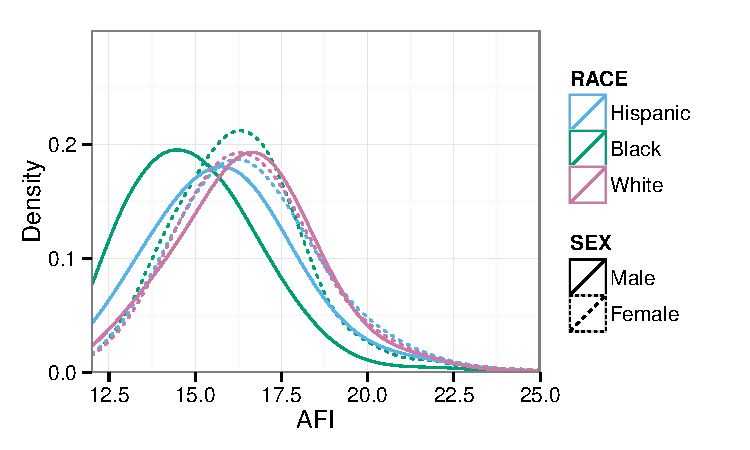
\includegraphics[width=.8\paperwidth]{figure/plot_afi_by_race_sex-1} 

\end{knitrout}
\end{center}
\pagebreak
%
\begin{center}
\captionof{figure}{Between Family Correlations}
\label{plot_between}
\begin{knitrout}
\definecolor{shadecolor}{rgb}{0.969, 0.969, 0.969}\color{fgcolor}
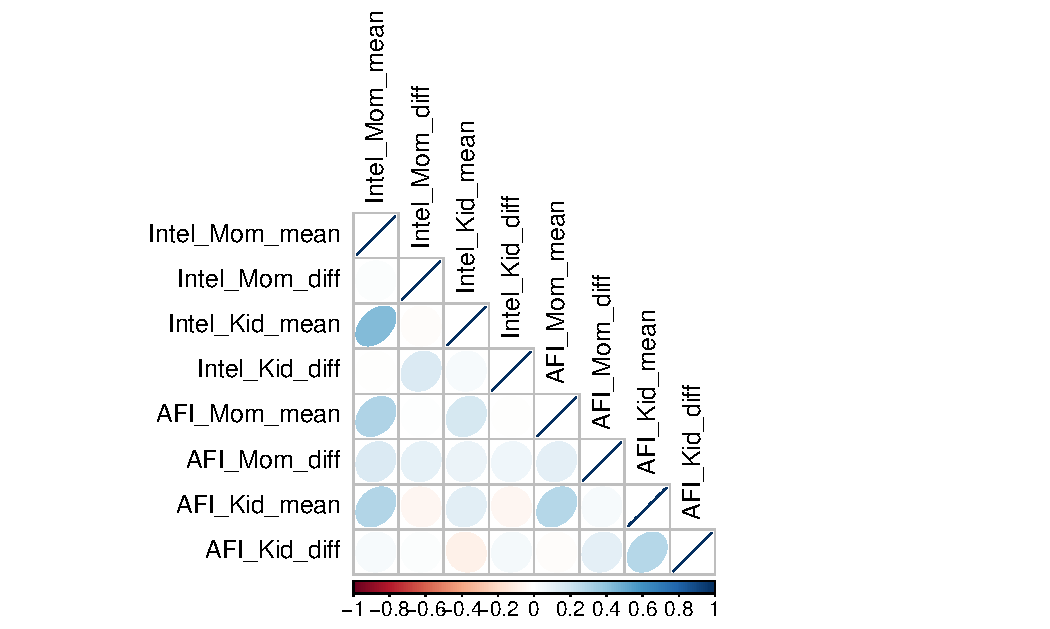
\includegraphics[width=1.1\paperwidth]{figure/plot_corplotmatrix_between-1} 

\end{knitrout}
\end{center}
\pagebreak
%
\begin{center}
\captionof{figure}{Within Family Correlations}
\label{plot_within}
\begin{knitrout}
\definecolor{shadecolor}{rgb}{0.969, 0.969, 0.969}\color{fgcolor}
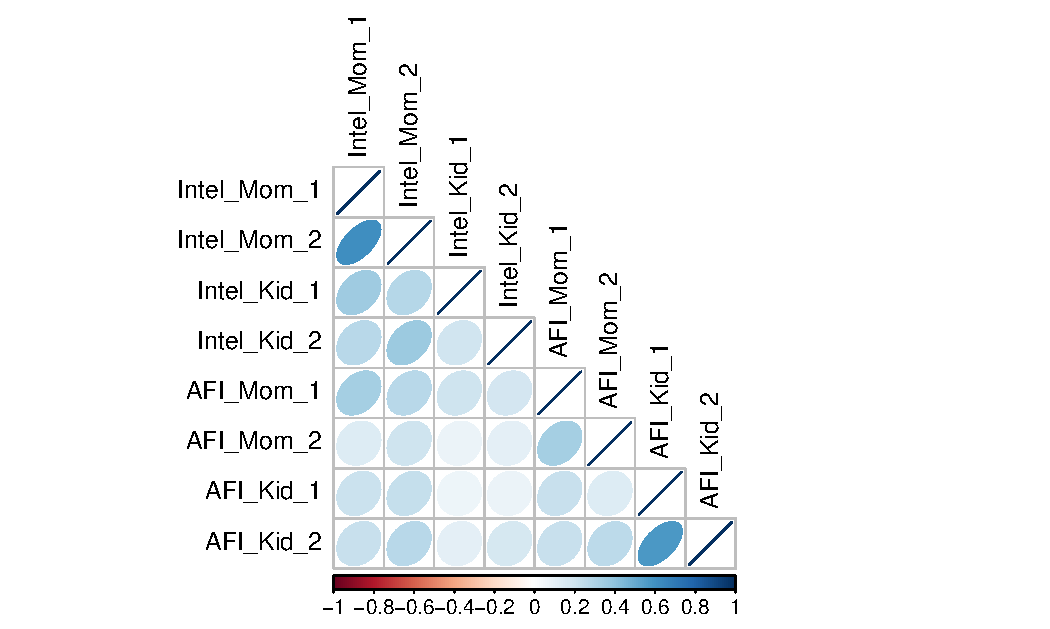
\includegraphics[width=1.1\paperwidth]{figure/plot_corplotmatrix_within-1} 

\end{knitrout}
\end{center}
%%%%%%%%%%%% References %%%%%%%%%%%%
\bibliography{Projects-AFI}
%
%%%%%%%%%%%% Appendix %%%%%%%%%%%%
\appendix\label{appen}
%
% Age 10.5 Replication
\section{Age 10.5 Replication}\label{appen10}
%% Measurement
%%% Measurement Model
\begin{longtable}{@{\extracolsep{5pt}}cc} 
\caption{Gen2 Measurement Model.}\label{table_gen2measurement_10}
\\[-1.8ex]\hline 
\hline \\[-1.8ex] 
 & g at Age 10.5 \\ 
\hline \\[-1.8ex] 
\partialinput{12}{34}{../Common/content/tables/table_g2_10measurement.tex}
\end{longtable}\pagebreak
%%%
%%% Factor Loadings
\begin{longtable}{@{\extracolsep{5pt}}cccccc} 
\caption{Gen2 Factor Loadings.}\label{table_g2loading_10}
\\[-1.8ex]\hline 
\hline \\[-1.8ex] 
 & Test & Estimate & S.E. & Est./.S.E. & P Value \\  
\hline \\[-1.8ex] 
\partialinput{12}{17}{../Common/content/tables/table_g2loading_10.tex}
\end{longtable}\pagebreak
%%
%% Between Family
\begin{landscape}
\subsection{Between Family Analyses}
%%%
%%% Mom -> Child
\begin{longtable}{@{\extracolsep{5pt}}lccc} 
\caption{Mean Gen1 Mean Intelligence $\rightarrow$ Gen2 Mean AFI}\label{table_Mean_Mom_Intelligence_Mean_Child_AFI_10}
\\[-1.8ex]\hline 
\hline \\[-1.8ex] 
 & \multicolumn{3}{c}{\textit{Dependent variable:} Average of Gen2 AFI} \\ 
\cline{2-4}
\partialinput{10}{22}{../Common/content/tables/table_Mean_Mom_Intelligence_Mean_Child_AFI_10.tex}
\end{longtable}\pagebreak
%%%
%%% Child -> Child
\begin{longtable}{@{\extracolsep{5pt}}lccc} 
\caption{Gen2 Mean Intelligence $\rightarrow$ Gen2 Mean AFI}\label{table_Mean_Child_Intelligence_Mean_Child_AFI_10}
\\[-1.8ex]\hline 
\hline \\[-1.8ex] 
 & \multicolumn{3}{c}{\textit{Dependent variable:} Average of Gen2 AFI} \\ 
\cline{2-4}
\partialinput{10}{22}{../Common/content/tables/table_Mean_Child_Intelligence_Mean_Child_AFI_10.tex}
\end{longtable}\pagebreak
%%%
%%% Mom Child -> Child
\begin{longtable}{@{\extracolsep{5pt}}lccc} 
\caption{Mean Joint Intelligence $\rightarrow$ Gen2 Mean AFI}\label{table_Mean_Joint_Intelligence_Mean_Child_AFI_10}
\\[-1.8ex]\hline 
\hline \\[-1.8ex] 
 & \multicolumn{3}{c}{\textit{Dependent variable:} Average of Gen2 AFI} \\ 
\cline{2-4}
\partialinput{10}{23}{../Common/content/tables/table_Mean_Joint_Intelligence_Mean_Child_AFI_10.tex}
\end{longtable}\pagebreak
%%
%% Within Family
\subsection{Within Family Analyses}
%%%
%%% Mom -> Child
\begin{longtable}{@{\extracolsep{5pt}}lccc} 
\caption{Gen1 Dif Intelligence $\rightarrow$ Gen2 Dif AFI}\label{table_Dif_Mom_Intelligence_Dif_Child_AFI_10}
\\[-1.8ex]\hline 
\hline \\[-1.8ex] 
 & \multicolumn{3}{c}{\textit{Dependent variable:} Difference in Gen2 Mean AFI} \\ 
\cline{2-4}
\partialinput{10}{24}{../Common/content/tables/table_Dif_Mom_Intelligence_Dif_Child_AFI_10.tex}
\end{longtable}\pagebreak
%%%
%%% Child -> Child
\begin{longtable}{@{\extracolsep{5pt}}lccc} 
\caption{Gen2 Dif Intelligence $\rightarrow$ Gen2 Dif AFI}\label{table_Dif_Child_Intelligence_Dif_Child_AFI_10}
\\[-1.8ex]\hline 
\hline \\[-1.8ex] 
 & \multicolumn{3}{c}{\textit{Dependent variable:} Difference in Gen2 Mean AFI} \\ 
\cline{2-4}
\partialinput{10}{24}{../Common/content/tables/table_Dif_Child_Intelligence_Dif_Child_AFI_10.tex}
\end{longtable}\pagebreak
%%%
%%% Mom Child -> Child
\begin{longtable}{@{\extracolsep{5pt}}lccc} 
\caption{Joint Dif Intelligence $\rightarrow$ Gen2 Dif AFI}\label{table_Dif_Joint_Intelligence_Dif_Child_AFI_10}
\\[-1.8ex]\hline 
\hline \\[-1.8ex] 
 & \multicolumn{3}{c}{\textit{Dependent variable:} Difference in Gen2 Mean AFI} \\ 
\cline{2-4}
\partialinput{10}{26}{../Common/content/tables/table_Dif_Joint_Intelligence_Dif_Child_AFI_10.tex}
\end{longtable}
\end{landscape}
%
% Age 11.5 Replication
\section{Age 11.5 Replication}\label{appen11}
%% Measurement
%%% Measurement Model
\begin{longtable}{@{\extracolsep{5pt}}cc} 
\caption{Gen2 Measurement Model.}\label{table_gen2measurement_11}
\\[-1.8ex]\hline 
\hline \\[-1.8ex] 
 & g at Age 11.5 \\ 
\hline \\[-1.8ex] 
\partialinput{12}{34}{../Common/content/tables/table_g2_11measurement.tex}
\end{longtable}\pagebreak
%%%
%%% Factor Loadings
\begin{longtable}{@{\extracolsep{5pt}}cccccc} 
\caption{Gen2 Factor Loadings.}\label{table_g2loading_11}
\\[-1.8ex]\hline 
\hline \\[-1.8ex] 
 & Test & Estimate & S.E. & Est./.S.E. & P.Value \\  
\hline \\[-1.8ex] 
\partialinput{12}{17}{../Common/content/tables/table_g2loading_11.tex}
\end{longtable}\pagebreak
%%
%% Between Family
\begin{landscape}
\subsection{Between Family Analyses}
%%%
%%% Mom -> Child
\begin{longtable}{@{\extracolsep{5pt}}lccc} 
\caption{Mean Gen1 Mean Intelligence $\rightarrow$ Gen2 Mean AFI}\label{table_Mean_Mom_Intelligence_Mean_Child_AFI_11}
\\[-1.8ex]\hline 
\hline \\[-1.8ex] 
 & \multicolumn{3}{c}{\textit{Dependent variable:} Average of Gen2 AFI} \\ 
\cline{2-4}
\partialinput{10}{22}{../Common/content/tables/table_Mean_Mom_Intelligence_Mean_Child_AFI_11.tex}
\end{longtable}\pagebreak
%%%
%%% Child -> Child
\begin{longtable}{@{\extracolsep{5pt}}lccc} 
\caption{Gen2 Mean Intelligence $\rightarrow$ Gen2 Mean AFI}\label{table_Mean_Child_Intelligence_Mean_Child_AFI_11}
\\[-1.8ex]\hline 
\hline \\[-1.8ex] 
 & \multicolumn{3}{c}{\textit{Dependent variable:} Average of Gen2 AFI} \\ 
\cline{2-4}
\partialinput{10}{22}{../Common/content/tables/table_Mean_Child_Intelligence_Mean_Child_AFI_11.tex}
\end{longtable}\pagebreak
%%%
%%% Mom Child -> Child
\begin{longtable}{@{\extracolsep{5pt}}lccc} 
\caption{Mean Joint Intelligence $\rightarrow$ Gen2 Mean AFI}\label{table_Mean_Joint_Intelligence_Mean_Child_AFI_11}
\\[-1.8ex]\hline 
\hline \\[-1.8ex] 
 & \multicolumn{3}{c}{\textit{Dependent variable:} Average of Gen2 AFI} \\ 
\cline{2-4}
\partialinput{10}{23}{../Common/content/tables/table_Mean_Joint_Intelligence_Mean_Child_AFI_11.tex}
\end{longtable}\pagebreak
%%
%% Within Family
\subsection{Within Family Analyses}
%%%
%%% Child -> Child
\begin{longtable}{@{\extracolsep{5pt}}lccc} 
\caption{Gen1 Dif Intelligence $\rightarrow$ Gen2 Dif AFI}\label{table_Dif_Mom_Intelligence_Dif_Child_AFI_11}
\\[-1.8ex]\hline 
\hline \\[-1.8ex] 
 & \multicolumn{3}{c}{\textit{Dependent variable:} Differences in Gen2 Mean AFI} \\ 
\cline{2-4}
\partialinput{10}{24}{../Common/content/tables/table_Dif_Mom_Intelligence_Dif_Child_AFI_11.tex}
\end{longtable}\pagebreak
%%%
%%% Child -> Child
\begin{longtable}{@{\extracolsep{5pt}}lccc} 
\caption{Gen2 Dif Intelligence $\rightarrow$ Gen2 Dif AFI}\label{table_Dif_Child_Intelligence_Dif_Child_AFI_11}
\\[-1.8ex]\hline 
\hline \\[-1.8ex] 
 & \multicolumn{3}{c}{\textit{Dependent variable:} Differences in Gen2 Mean AFI} \\ 
\cline{2-4}
\partialinput{10}{24}{../Common/content/tables/table_Dif_Child_Intelligence_Dif_Child_AFI_11.tex}
\end{longtable}\pagebreak
%%%
%%% Mom Child -> Child
\begin{longtable}{@{\extracolsep{5pt}}lccc} 
\caption{Dif Joint Intelligence $\rightarrow$ Gen2 Dif AFI}\label{table_Dif_Joint_Intelligence_Dif_Child_AFI_11}
\\[-1.8ex]\hline 
\hline \\[-1.8ex] 
 & \multicolumn{3}{c}{\textit{Dependent variable:} Differences in Gen2 Mean AFI} \\ 
\cline{2-4}
\partialinput{10}{26}{../Common/content/tables/table_Dif_Joint_Intelligence_Dif_Child_AFI_11.tex}
\end{longtable}
\end{landscape}
%
\end{document}
